% ============================================================
% 2A
% ============================================================
\section{Task 2A: Software Prefetching}

\subsection{Experimental Setup}
\begin{itemize}
    \item CPU: Intel x86 architecture (Tested on HP Pavilion Laptop)
    \item Matrix dimensions: $128 \times 128$ to $2048 \times 2048$
    \item Prefetch distances: Swept across multiple values; 32 floats (2 cache lines) identified as optimal
    \item Cache fill levels: T0, T1, T2, NTA
    \item Performance counters: \texttt{instructions}, \texttt{cpu\_core/L1D.REPLACEMENT/}, \texttt{l2\_rqsts.miss}, \texttt{LLC-load-misses}, \texttt{sw\_prefetch\_access.any}
    \item Number of runs: 1 warmup, 3 timed repetitions
\end{itemize}

\subsection{Matrix Size Analysis}
As the matrix size increases from $128 \times 128$ up to $2048 \times 2048$, the measured benefit of software prefetching increases in both hardware-prefetcher configurations.

When hardware prefetchers are OFF, the speedup rises from $1.69\times$ at $N=128$ to $2.08\times$ at $N=2048$. With hardware prefetchers ON, the measured gains are similar, from $1.80\times$ to $2.07\times$. In the NT layout, the inner $K$ accesses are contiguous in both operands, but the kernel still has multiple concurrent streams and repeatedly traverses large rows. These results suggest that explicit prefetching can provide additional benefit even when hardware prefetching is enabled.

\subsection{Execution Time and Speedup}
$$
\text{Speedup} =
\frac{\text{Execution Time without Software Prefetching}}
{\text{Execution Time with Software Prefetching}}
$$

\begin{table}[H]
\centering
\caption{Best Software prefetching configurations (HW Prefetch OFF vs ON)}
\begin{tabular}{l|c|c|c||c|c|c}
\toprule
& \multicolumn{3}{c||}{\textbf{HW Prefetch OFF}} & \multicolumn{3}{c}{\textbf{HW Prefetch ON}} \\
Size & Distance/Hint & Time (ms) & Speedup & Distance/Hint & Time (ms) & Speedup \\
\midrule
$128 \times 128$   & 16 / T1 & 0.4130   & 1.6996$\times$ & 16 / NTA & 0.4116   & 1.8040$\times$ \\
$256 \times 256$   & 16 / T1 & 3.4508   & 1.8003$\times$ & 16 / T1  & 3.4766   & 1.7553$\times$ \\
$512 \times 512$   & 16 / T0 & 28.1323  & 1.8825$\times$ & 64 / T1  & 28.2706  & 1.9187$\times$ \\
$1024 \times 1024$ & 16 / T2 & 227.5796 & 1.9456$\times$ & 256 / T2 & 228.7783 & 2.0067$\times$ \\
$2048 \times 2048$ & 16 / T2 & 1868.4863& 2.0849$\times$ & 64 / T1  & 1864.7300& 2.0702$\times$ \\
\bottomrule
\end{tabular}
\end{table}

\begin{figure}[H]
\centering
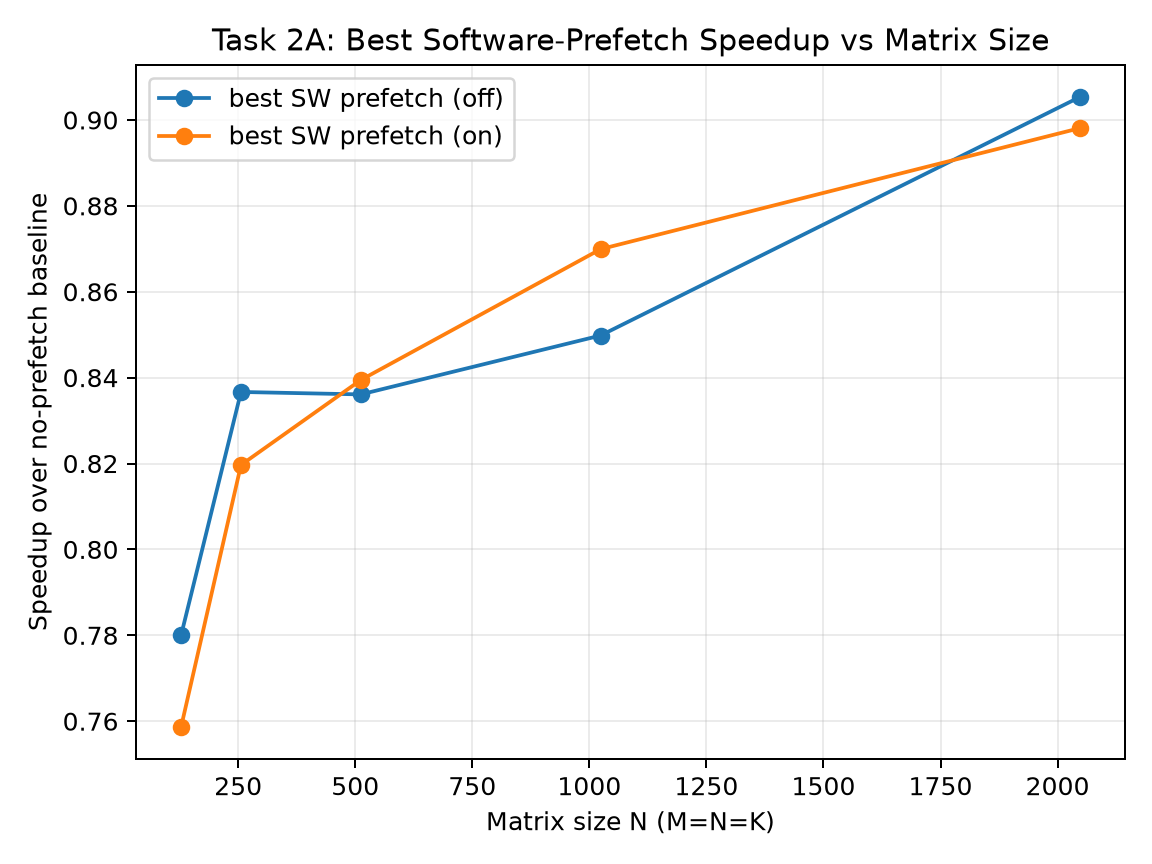
\includegraphics[width=0.75\linewidth]{plots/task2a/task2a_speedup_vs_size.png}
\caption{Software prefetching speedup vs. matrix size (comparing HW prefetcher states).}
\end{figure}

\subsection{CPU Metrics}
\begin{figure}[H]
    \centering
    \begin{subfigure}{0.48\textwidth}
        \centering
        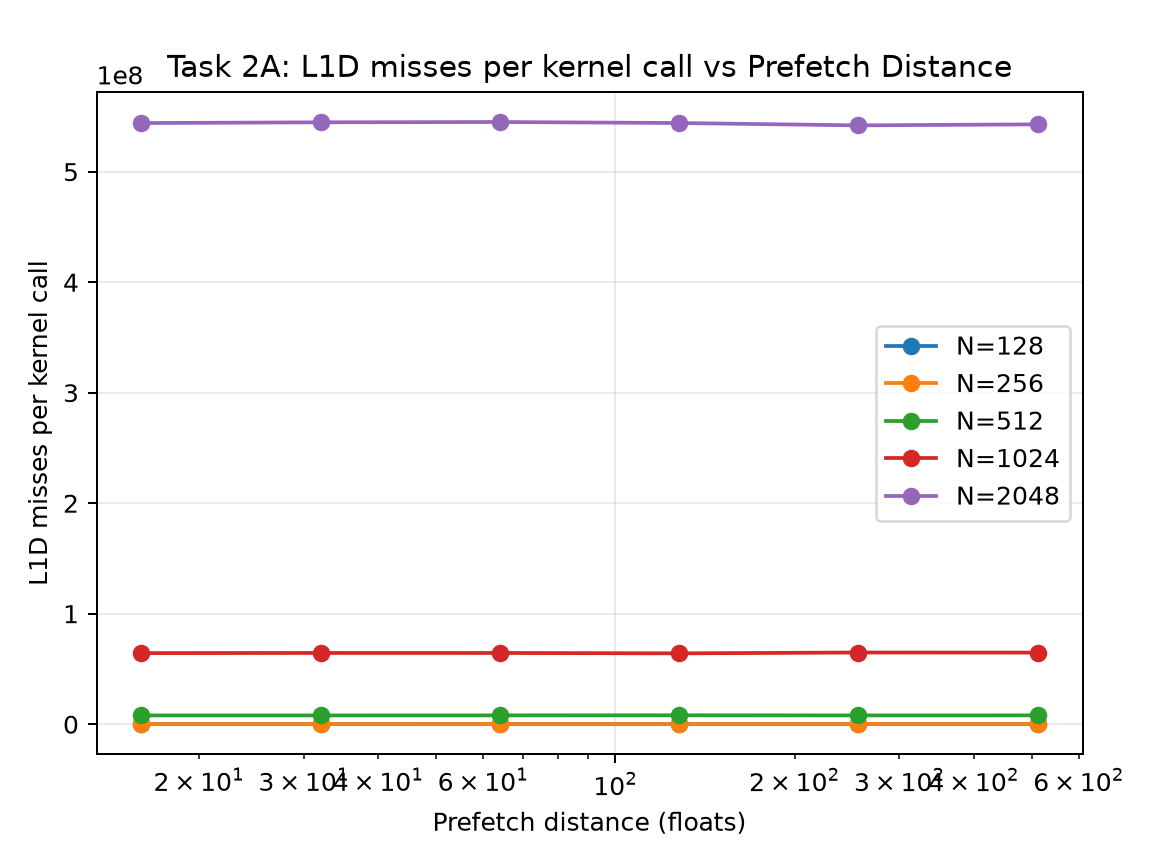
\includegraphics[width=\linewidth]{plots/task2a/task2a_l1d_misses_vs_distance.png}
        \caption{L1D Misses vs Prefetch Distance}
    \end{subfigure}
    \hfill
    \begin{subfigure}{0.48\textwidth}
        \centering
        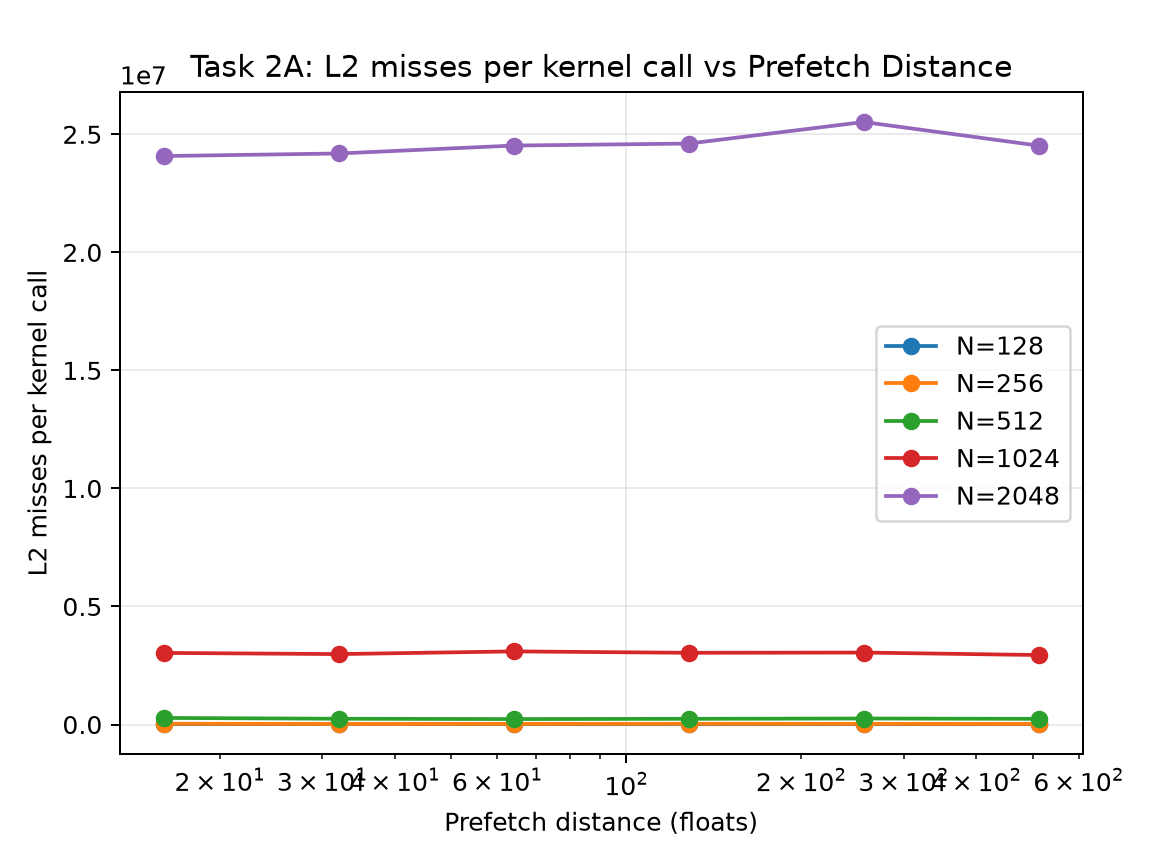
\includegraphics[width=\linewidth]{plots/task2a/task2a_l2_misses_vs_distance.png}
        \caption{L2 Misses vs Prefetch Distance}
    \end{subfigure}
    \vspace{1em}
    \begin{subfigure}{0.48\textwidth}
        \centering
        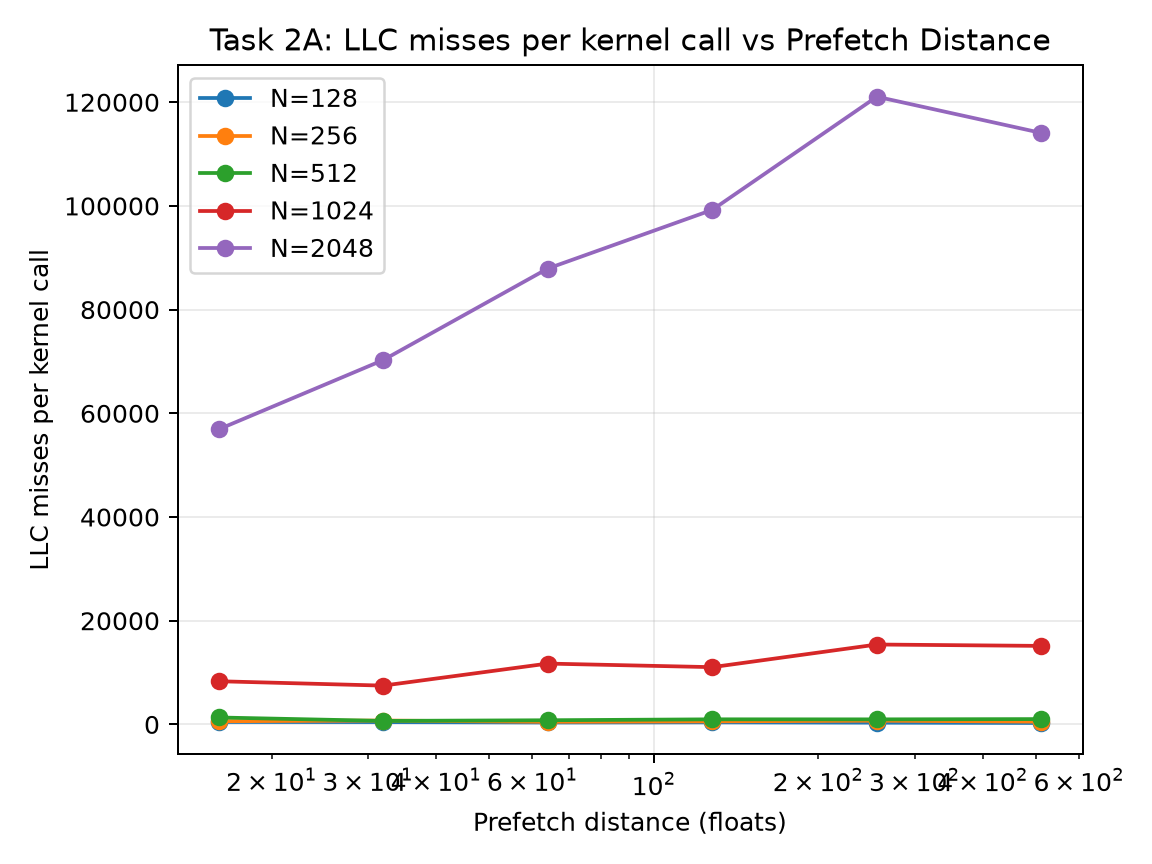
\includegraphics[width=\linewidth]{plots/task2a/task2a_llc_misses_vs_distance.png}
        \caption{LLC Misses vs Prefetch Distance}
    \end{subfigure}
    \hfill
    \begin{subfigure}{0.48\textwidth}
        \centering
        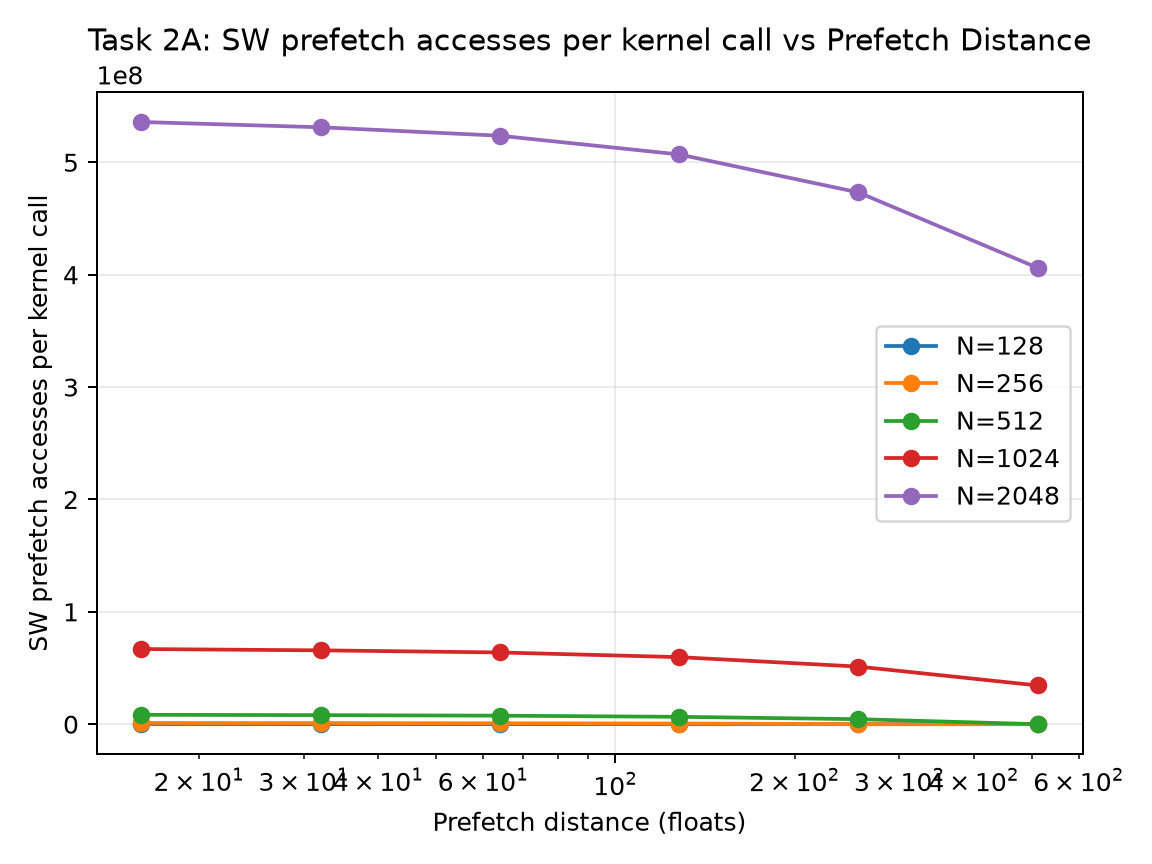
\includegraphics[width=\linewidth]{plots/task2a/task2a_sw_prefetch_access_vs_distance.png}
        \caption{SW Prefetch Accesses vs Distance}
    \end{subfigure}
    \caption{Hardware cache metrics behavior under varying prefetch distances.}
\end{figure}

\subsection{Prefetch Distance}
The prefetch distance determines how far ahead the CPU requests data. Based on the geometric mean across all evaluated sizes, 32 floats (two 64-byte cache lines) gave the best global result. This is distinct from the best configuration at an individual size, which can use another distance. Requests that are too far ahead can add cache pressure or arrive before the data is used.

\begin{figure}[H]
\centering
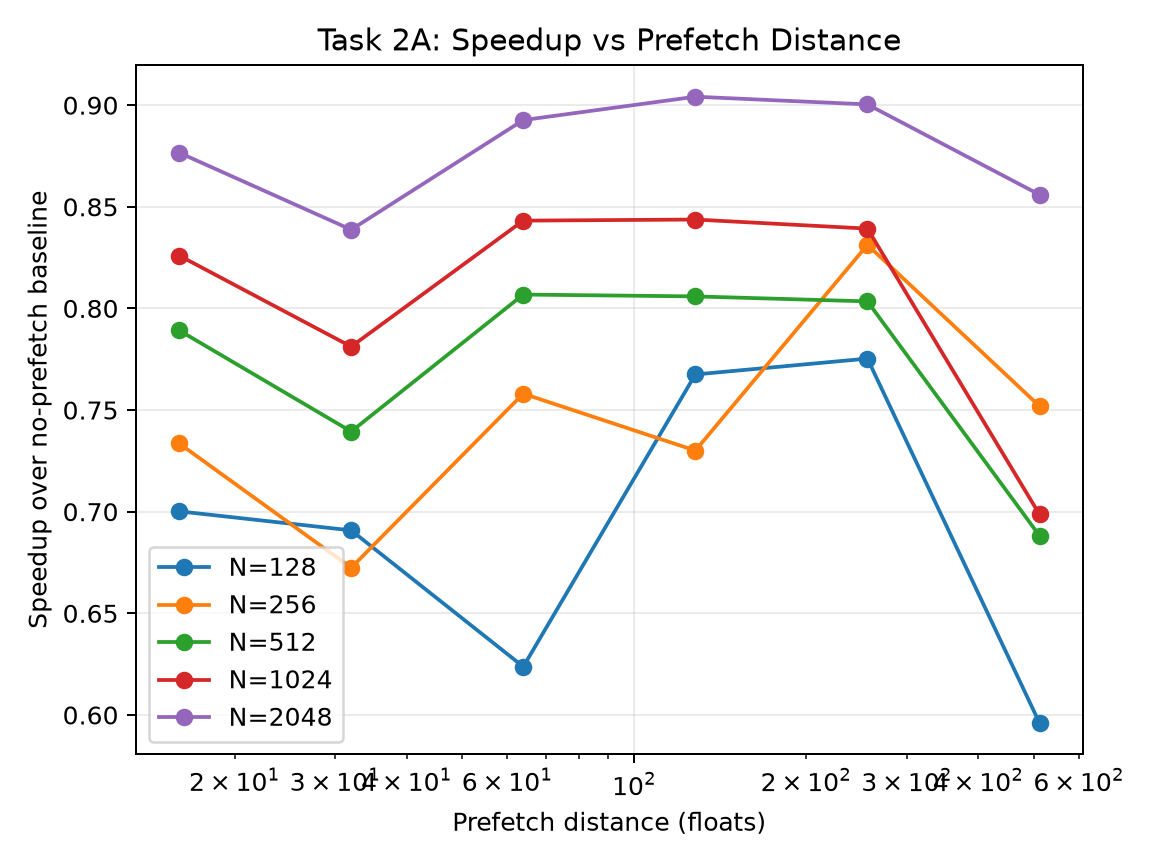
\includegraphics[width=0.75\linewidth]{plots/task2a/task2a_prefetch_distance.png}
\caption{Speedup over baseline across varying prefetch distances.}
\end{figure}

\subsection{Cache Fill Level}
The locality hint expresses the expected temporal reuse of prefetched data; it does not guarantee placement in a particular cache level. Taking the geometric mean across all matrix sizes, \texttt{T1} provided the best overall result. The result is consistent with lower L1 cache pressure than \texttt{T0}, although exact behavior is microarchitecture-dependent.

\begin{figure}[H]
\centering
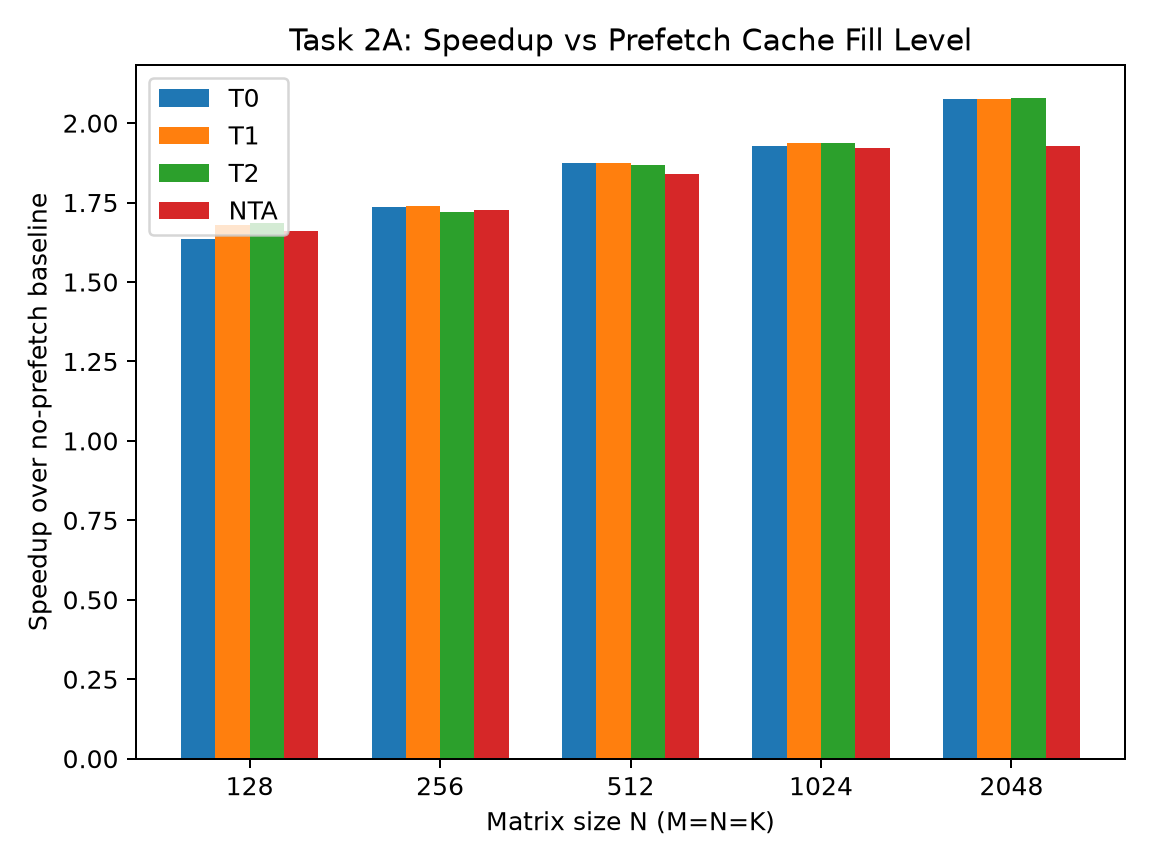
\includegraphics[width=0.75\linewidth]{plots/task2a/task2a_prefetch_level.png}
\caption{Speedup over baseline across varying cache fill levels.}
\end{figure}

\subsection{Hardware Prefetchers}
The results show that software prefetching provided additional benefit with hardware prefetchers enabled. Although the inner $K$ streams are linear, the blocked kernel has several active streams and reuse patterns, so hardware prefetching need not hide every data-delivery delay. The best observed speedup with hardware prefetching enabled was $\sim 2.07\times$.

\begin{figure}[H]
\centering
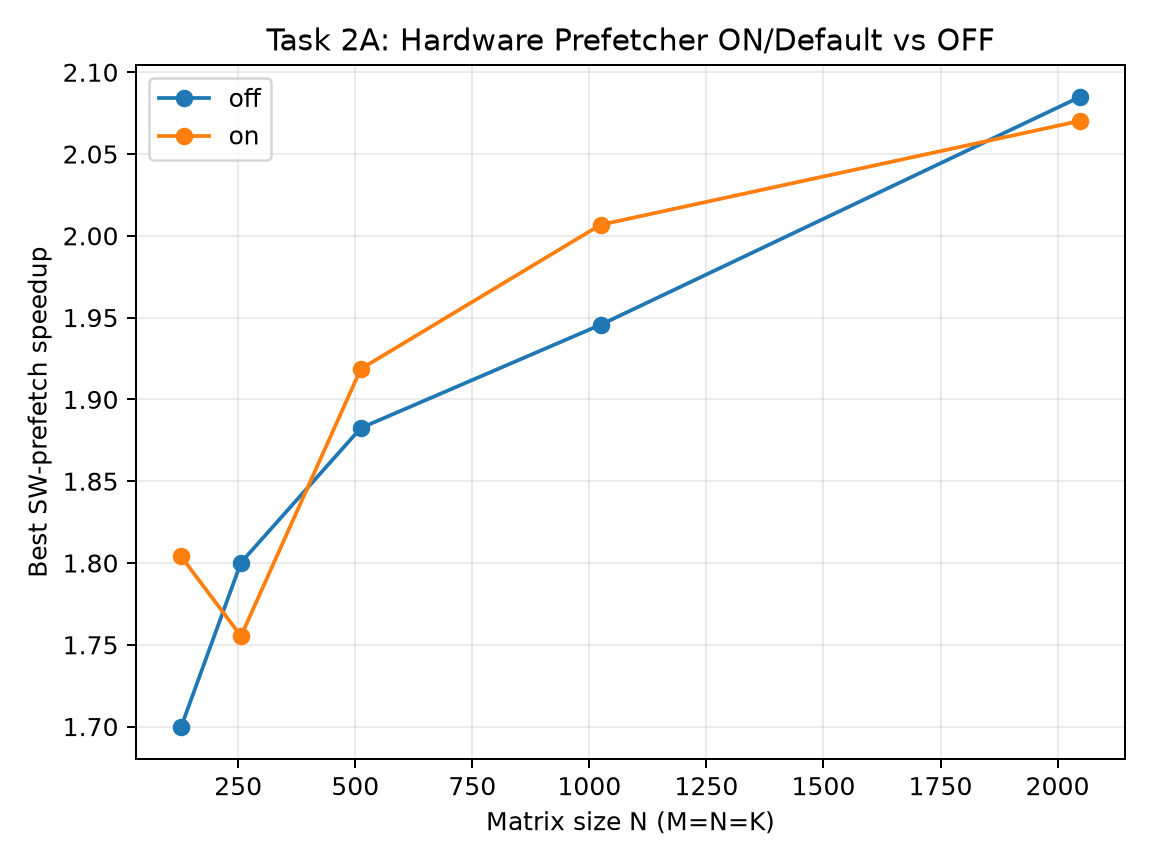
\includegraphics[width=0.75\linewidth]{plots/task2a/task2a_hw_prefetch_on_off.png}
\caption{Hardware prefetcher ON vs OFF comparison.}
\label{fig:hw_prefetch}
\end{figure}

\subsection{Questions}
\begin{enumerate}
    \item \textbf{What trend do you observe in speedup with different matrix sizes?} \\
    In these measurements, speedup increases with matrix size in both hardware-prefetcher configurations, from about $1.7\times$ at $N=128$ to about $2.08\times$ at $N=2048$. This trend is consistent with data-delivery delays becoming a larger fraction of execution time as the working set grows.
    
    \item \textbf{What is the best prefetch distance?} \\
    Based on the geometric mean across all evaluated sizes, 32 floats (which translates to 2 cache lines) is the optimal prefetch distance.
    
    \item \textbf{At what cache fill level do you achieve the maximum speedup?} \\
    The \texttt{T1} hint achieved the maximum geometric-mean speedup. It requests lower temporal locality than \texttt{T0}; the actual cache response is microarchitecture-dependent.
\end{enumerate}
